\documentclass{assignment}
\usepackage[utf8]{inputenc}
\usepackage[T1]{fontenc}
\usepackage{hyperref}
\usepackage{listings}

\begin{document}
	
	\assignmentTitle{Claudio Iván Esparza Castañeda}{Luis Alberto Balam Guzmán}{./Logo.png}{Maestría en Sistemas Embebidos}{Programación y Procesamiento de Datos}{5B. Práctica de paralelismo en Python}
	\section*{Objetivo}
	Con la imposibilidad que representa tener que procesar grandes cantidades de información en un medio con pocos recursos, refiriéndonos en este caso a la Raspberry Pi Pico, surge la necesidad de contar con sistemas híbridos: control en el sistema embebido, y procesamiento en la computadora.\\
	En sistemas modernos, se cuenta con controladores y procesadores con múltiples núcleos. Eso, además de arquitecturas basadas en pipeline permiten manejar múltiples operaciones en un solo chip, empleando distintas operaciones.\\
	En esta práctica se aborda el el uso de procesamiento simultáneo con la intención de verificar cómo se realiza con archivos de diversas fuentes. Con la potencia de cálculo de las computadoras actuales, es probable que no se note una diferencia significativa en este caso a comparación de hacerlo en un solo proceso, sin embargo sirve de ilustración para cuando se requiera en aplicaciones reales.
	
	\section*{Descipción de la solución}
	Se dividieron las responsabilidades de los distintos procesos. Por un lado, el archivo {\tt analisis.py} contiene la información relacionada a los cálculos, limitándose a las funciones que se dividirán en los distintos procesos. El archivo {\tt graficas.py} se describe a sí mismo, y contiene las funciones que dan el estilo a las gráficas procedentes de los datos que se procesan. Por último, el archivo {\tt main.py} orquesta estos dos y contiene la inicialización de las entradas.\\
	Se sigue usando el archivo {\tt funciones.py} de tareas anteriores, con el objetivo de hacer algunas validaciones.
	\begin{figure}[htbp]
		\centering
		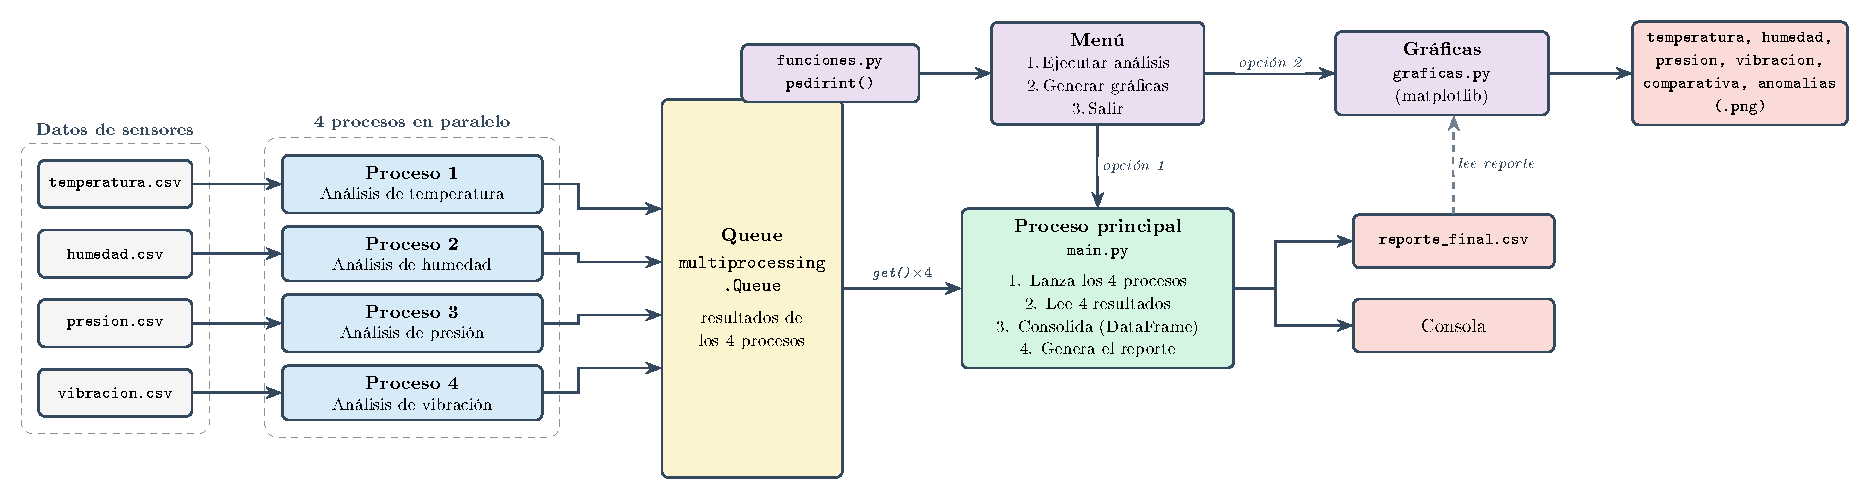
\includegraphics[width=\textwidth]{Figuras/1}
		\caption{Diagrama de la solución}
		\label{fig:1}
	\end{figure}
	\section*{Metodología}
	El tratamiento de las señales se limita a usar NumPy, pues se solicitan cálculos estadísticos sobre vectores. Se establece el factor  de anomalía, que permite discernir la desviación necesaria para clasificarse como tal. Las anomalías se terminan guardando en un vector que conserva los índices, para posteriormente incorporar ambas cosas en las gráficas del sensor.\\
	El programa emplea la misma base anterior para el menú.
	\section*{Capturas de ejecución}
	\begin{figure}[htbp]
		\centering
		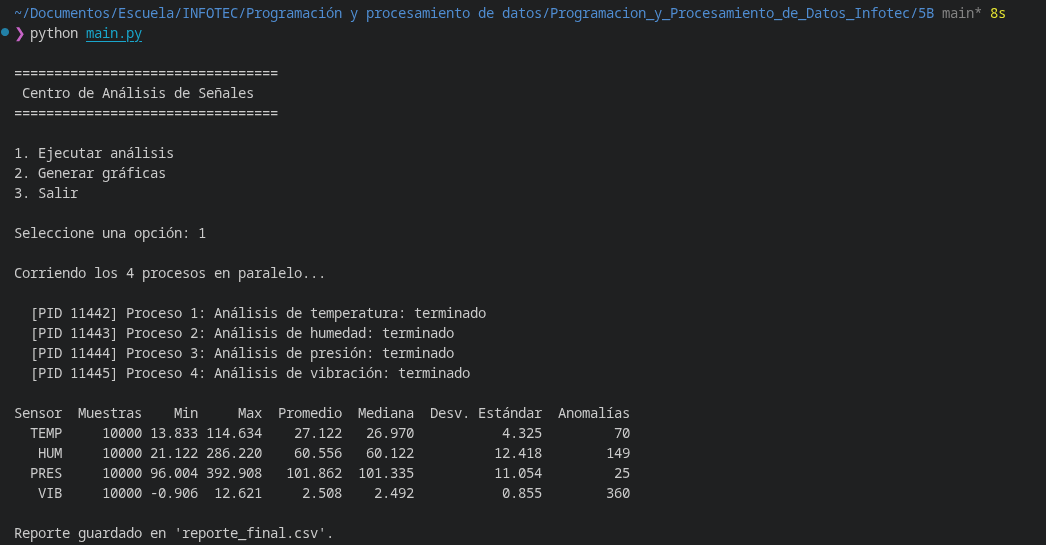
\includegraphics[width=\textwidth]{Figuras/2}
		\caption{Ejecución del programa. Opción 1 seleccionada}
		\label{fig:2}
	\end{figure}
	\begin{figure}[htbp]
		\centering
		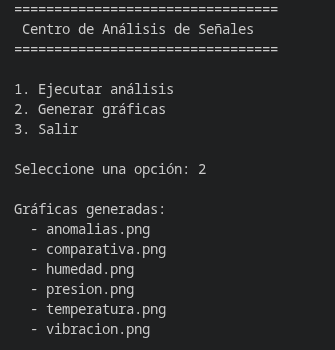
\includegraphics[width=0.5\textwidth]{Figuras/3}
		\caption{Ejecución del programa. Opción 2 seleccionada}
		\label{fig:3}
	\end{figure}
	\begin{figure}[htbp]
		\centering
		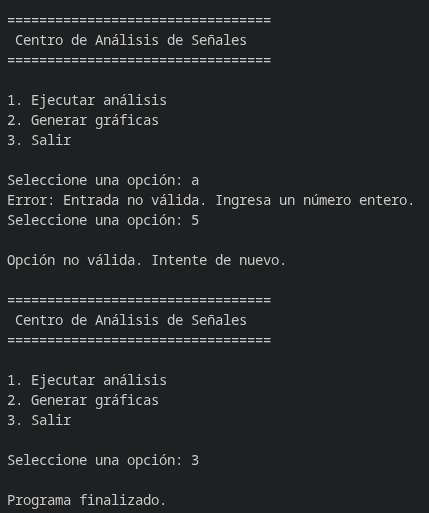
\includegraphics[width=0.5\textwidth]{Figuras/4}
		\caption{Ejecución del programa. Validación de entero y de rango de la opción. Opción de salida correcta}
		\label{fig:4}
	\end{figure}
	\begin{figure}[htbp]
		\centering
		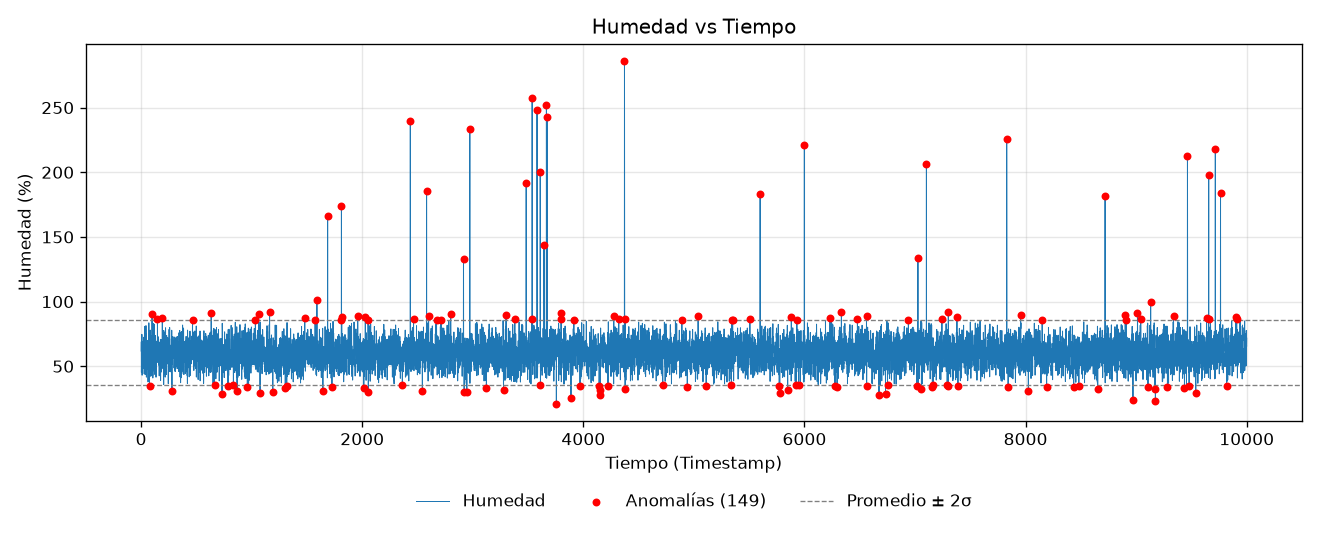
\includegraphics[width=\textwidth]{Figuras/5}
		\caption{Datos de humedad}
		\label{fig:5}
	\end{figure}
	\begin{figure}[htbp]
		\centering
		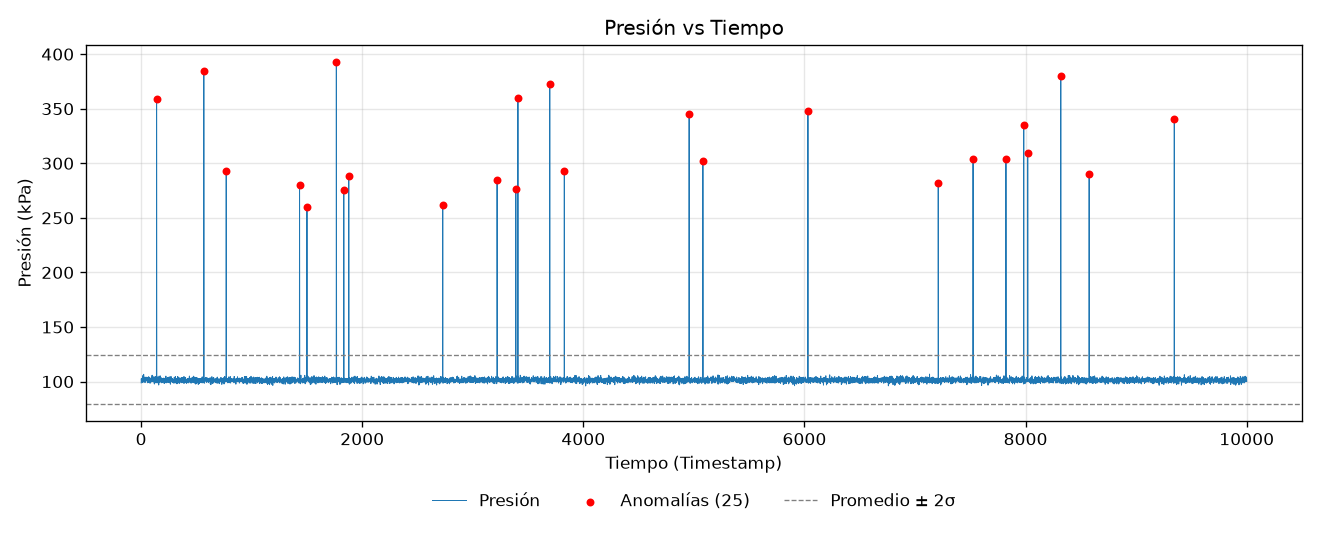
\includegraphics[width=\textwidth]{Figuras/6}
		\caption{Datos de presión}
		\label{fig:6}
	\end{figure}
	\begin{figure}[htbp]
		\centering
		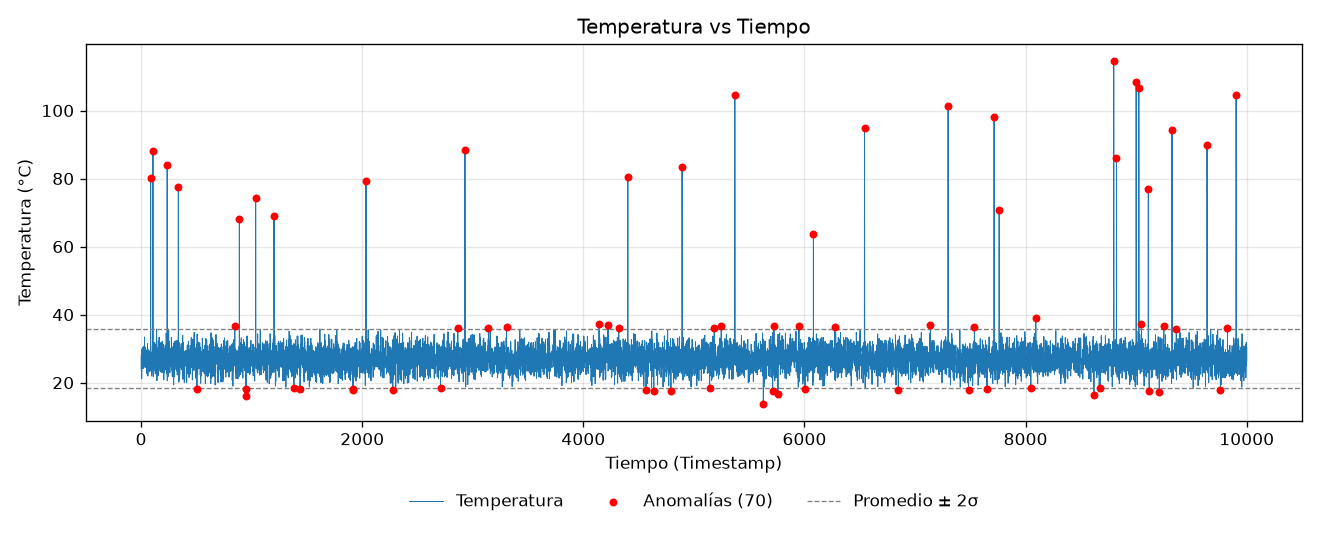
\includegraphics[width=\textwidth]{Figuras/7}
		\caption{Datos de temperatura}
		\label{fig:7}
	\end{figure}
	\begin{figure}[htbp]
		\centering
		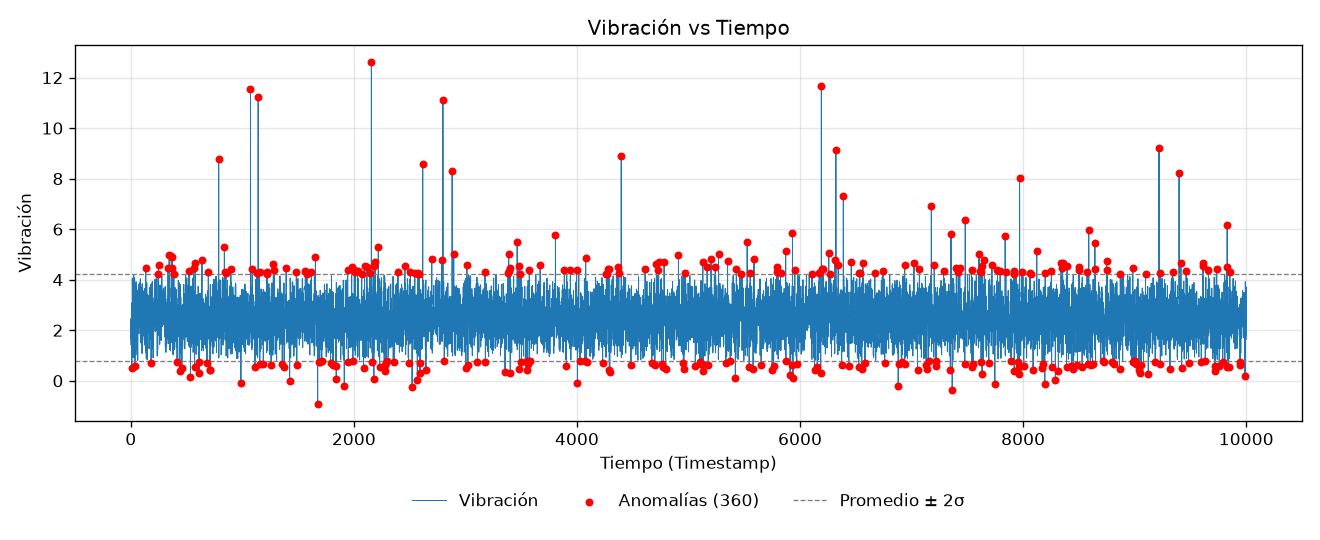
\includegraphics[width=\textwidth]{Figuras/8}
		\caption{Datos de vibración}
		\label{fig:8}
	\end{figure}
	\begin{figure}[htbp]
		\centering
		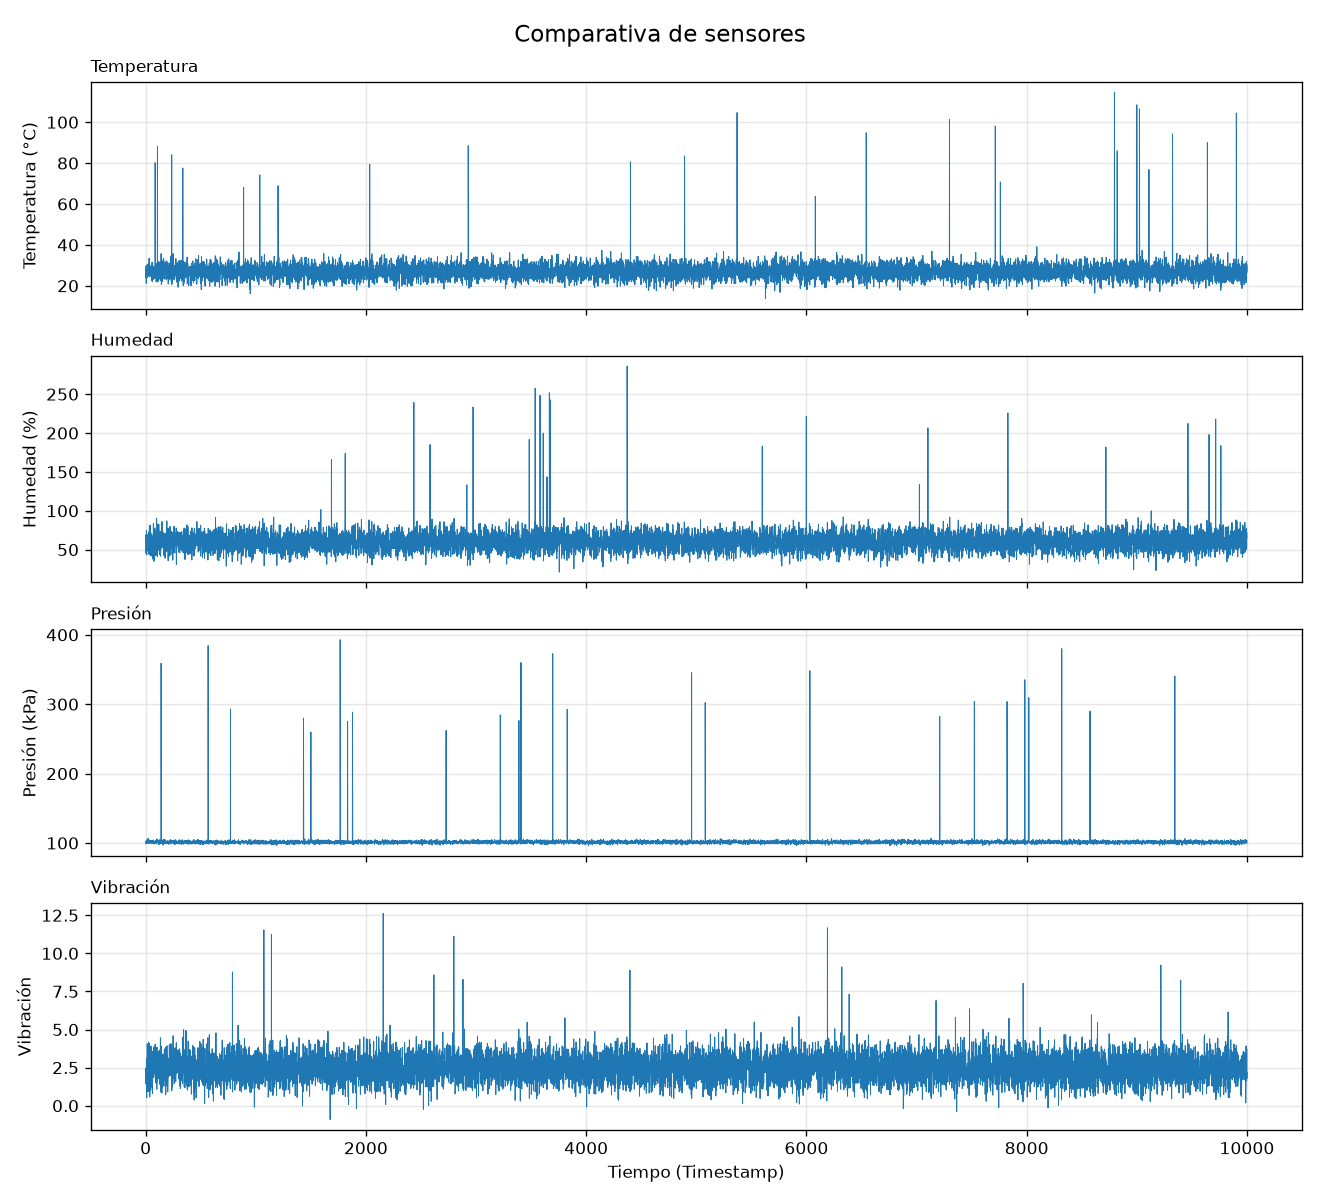
\includegraphics[width=\textwidth]{Figuras/9}
		\caption{Comparativa de los distintos sensores}
		\label{fig:9}
	\end{figure}
	\begin{figure}[htbp]
		\centering
		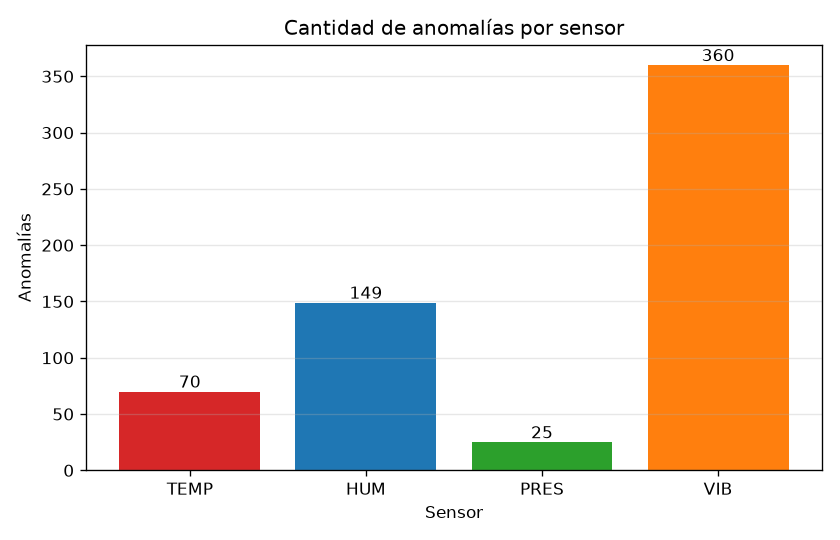
\includegraphics[width=\textwidth]{Figuras/10}
		\caption{Cantidad de anomalías por sensor}
		\label{fig:10}
	\end{figure}
	\clearpage
	\section*{Conclusiones}
		Como mencioné antes, con el poder de cálculo que contienen las computadoras modernas, es probable que no se vea una diferencia en realizar este ejercicio pequeño en procesos divididos personalmente o con lo que disponga el CPU.\\
		Otra cuestión que habría que plantear es que ahora las computadoras podrían incorporar además GPU, NPU, TPU, o las unidades de procesamiento de moda, por lo que dependiendo del tipo de operaciones necesarias se implicaría contar con un análisis de la mejor manera de optimizar el trabajo cuando se cuenta con estas condiciones,\\
		Con estas cuestiones en mente, conviene detenerse a analizar qué sería necesario separara "a mano" en los procesos, y cuáles cosas se deben dejar al sistema operativo. También los alcances en las computadoras modernas que cuentan con tales recursos.\\
		La carpeta en el repositorio de este proyecto es: \href{https://github.com/clivan/Programacion_y_Procesamiento_de_Datos_Infotec/5B}{Programación y procesamiento de Datos}.	
\end{document}
